\NeedsTeXFormat{LaTeX2e}
\documentclass[12pt]{article}
\usepackage[pdftex]{color,graphicx}
\usepackage{authblk}
\usepackage{amsmath,amsfonts}
\usepackage{graphicx,caption,subcaption}
\numberwithin{equation}{section}
\begin{document}

\title{\bf{Integrated Data Analysis of the DIII-D Density Profile}}
\author[1]{L. Stagner}
\author[1]{W.W. Heidbrink}
\author[2]{MA Van Zeeland}
\author[2]{L. Zeng}
\affil[1]{\small{University of California--Irvine, Irvine, California, USA}}
\affil[2]{\small{General Atomics, P. O. Box 85608, San Diego, California 92186-5608, USA}}
\date{}
\maketitle
\begin{abstract}
\end{abstract}
\section{Introduction}
Introstuff

\section{Integrated Data Analysis}
As fusion experiments expand, so does the number of diagnostics used to 
probe the underlying physics. With the increase in diagnostics the 
number of interrelations among the diagnostics increases accordingly. 
While each diagnostic can act independently it is often advantageous to 
combine the data sets to acquire the most accurate result that is 
consistent with all the information available. This causes difficulties 
when trying to combine multiple data sets that cover complementary 
areas of interest. Bayesian data analysis give a comprehensive, 
scalable, and automated framework for combining complementary 
diagnostics.    
\subsection{The Bayesian perspective}
Bayesian statistics differs from the prevailing frequentist statistics 
that is taught in most introductory courses. The difference between the 
two views is in the definition of probability. In the Bayesian 
perspective, probability represented a degree of belief or plausibility 
that an event was true, based on the information available. This school 
of thought is opposed to frequentist view that probability is a long 
run relative frequency with which the event occurs, given infinitely 
many repeated experimental trials.\cite{von2011bayesian}

While the frequentist view is seemingly more objective, it is limited 
in its straightforward application since some things cannot have long 
run relative frequencies and, as a result, cannot be analyzed by 
probability theory. For instance a constant, such as the mass of an 
object, cannot be analyzed by a straightforward application of the 
frequentist definition of probability as a long run relative frequency. 
To use the frequentist view you first have to relate the mass to the 
data through some function called the \emph{statistic}. Since 
statistic is subject to random noise it becomes the random variable to 
which the rules of probability can then be applied. The issue with this 
approach is that there is no natural way of choosing the best 
statistic.\cite{sivia2006data} The founders of the field have a 	
plethora of ad hoc rules and tests to determine which statistic should 
be used in any situation. These rules and tests hides much of the 	
mechanics and assumptions inherent in the analysis and the consequences 
can often turn up at the worst possible moments.

The bayesian definition has no such difficulty since nearly anything 
can be thought of as a probability and the framework explicitly 
formulates all assumptions. That is not to say that it is without its 
issues. The frequentist view is often much easier to use because it 
hides most of the difficulties from the user. In bayesian statistics 
you have to be very careful with the assumptions that are made since it 
can drastically affect the results. Also, the calculation of optimal 
parameters is also a challenging numerical exercise in Bayesian 
statistics. It was partially for this reason that the frequentist view 
arose into prominence. It was only in the mid 20\textsuperscript{th} 
century with the advent of computers and efficient sampling algorithms 
that Bayesian statistics has begun its resurgence. In recent years 
Bayesian analysis has become essential to many scientific fields such 
as cosmology and artificial intelligence.\cite{von2011bayesian}
\subsection{Mathematical Formulation}
In 1946, Richard Cox began to formulate the rules for logical and consistent
reasoning by considering how we might quantify our beliefs about the truth of 
an event or object. He concluded that the real numbers we attached to our
beliefs followed the rules of probability:\cite{sivia2006data} 
\begin{equation} \label{eq:sumrule}
	prob(X|I) + prob(\overline{X}|I) = 1
\end{equation}
and 
\begin{equation} \label{eq:productrule}
	prob(X,Y|I) = prob(X|Y,I) \times prob(Y|X,I)
\end{equation}
Here $\overline{X}$ denotes that $X$ is false and the vertical bar `$|$' means `given'. 
All the probabilities are conditional on $I$ to denote the relevant background information 
available, since there is no such thing as an absolute probability. 

Equation \ref{eq:sumrule} and \ref{eq:productrule} are called the sum and product 
rules, respectively. The sum and product rule form the basic equations of probability 
theory. From these two rules we can derive the core equations used in bayesian 
statistics: Bayes' theorem
\begin{equation} \label{eq:bayes1}
	prob(X|Y,I) = \frac{prob(Y|X,I) \times prob(X|I)}{prob(Y|I)}
\end{equation}
and marginalization.
\begin{equation} \label{eq:marginalization}
	prob(X|I) = \int_{-\infty}^{\infty}{(X,Y|I)dY}
\end{equation}

The power behind Bayes theorem can best be recognized with a change of notation. 
\begin{align}\label{eq:bayes2}
	prob(&hypothesis|\{data\},I) =  \nonumber \\ 
	& \frac{prob(\{data\}|hypothesis,I) \times prob(hypothesis|I)}{prob(\{data\}|I)}
\end{align}
or as denoted in most parameter estimation problems:
\begin{equation} \label{eq:bayes3}
\mathcal{P}(\vec{\alpha}|\vec{d},I) = \frac{\mathcal{L}(\vec{d}|\vec{\alpha},I)\pi(\vec{\alpha}|I)}{\mathcal{Z}(\vec{d}|I)}
\end{equation}
where $\vec{\alpha}$ are the parameters to be inferred.
The terms in the above equation have formal names. $prob(hypothesis|I)$ is 
called the \emph{prior}. The prior encodes the current state of knowledge about the parameters before 
we have analyzed any new data. 
When we have acquired new information the prior is modified by the first term, $prob(\{data\}|hypothesis,I)$ called the 
\emph{likelihood}.
The product of the likelihood and the prior give $prob(hypothesis|\{data\},I)$, 
which is called the \emph{posterior}. The posterior encodes our final state of knowledge 
after all the data has been incorporated.
The maximum value of the posterior gives us the best estimate of the parameters we trying to infer.
The last term, $prob(\{data\}|I)$, is called the \emph{evidence} or \emph{marginal likelihood}. In parameter estimation problems the 
evidence can be ignored since it is essentially a normalization constant. However, in model comparison problems it is of vital 
importance.
\subsection{Choosing the Best Prior}
It was noted earlier that one has to be extra careful with the assumptions that are made prior 
to incorporating data. Quite fittingly, these assumptions are encoded in the choice of prior. 
This process can be difficult and if often done incorrectly. In order to choose the best prior 
three main schools of thought for choosing priors have been developed. 

The first school of thought is to choose a prior that expresses specific, definite information about a parameter.
If, for instance, a parameter is known, through past experience or expert testimony, to have a value 
around $1 \pm 0.2$ with upper bound of $2$. It would not be uncommon for someone to assign a prior that is a Gaussian with a mean of 
$1$ and standard deviation of $0.2$ that is zero for values greater than $2$. Informative priors are both a major advantage and can 
also be a major pitfall. If our prior knowledge was incorrect and the upper bound is around $5$, depending on the amount of data, we 
may have biased the posterior such that it doesn't reflect the truth. We must then be careful not to bias our results without proper 
justification. Informative priors also suffer from the fact that there is not a well defined procedure for choosing them. 

The second school of thought is to be as non-informative as possible. This method should 
be used when we have no prior information about the parameter in question. The most common type of non-informative prior 
is called the Jeffreys' Prior. The key property of the Jeffreys' Prior is that it is invariant under re-parametrization. 
The Jeffreys' prior is defined as 
\begin{equation} \label{eq:jefferys}
	\pi(\vec{\alpha}) \propto \sqrt{det \,\mathcal{I}(\vec{\alpha})}
\end{equation}
where $\mathcal{I}$ is the Fisher information. One of the main problems with the Jefferys' Prior is that it can be 
improper in the sense that it cannot normalizable to one (although there are ways around this). Improper priors should 
not be used since it can lead to paradoxes.\cite{von2011bayesian}
The Jefferys' Prior is also sometimes impossible to calculate and is therefore of limited use.

The third school of thought is to choose the prior that has the largest Shannon information entropy that is still consistent with the 
given testable information. The idea is that entropy is a measure of ``uninformativeness'' so picking the most `uninformative' prior 
that is still consistent with testable information would be the best choice. Mathematically, this the constrained optimization 
problem:
\begin{equation} \label{eq:maxent}
	Q = -\int \pi(x) log(\frac{\pi(x)}{m(x)})dx - \lambda C(x) 
\end{equation}
where $p(x)$ is the prior, $m(x)$ is the Lebesgue measure which ensures invariance under transformation, $\lambda$ is the Lagrange 
multiplier, and $C(x)$ is the constraint function. For example, if we knew the mean of a parameter, using the 
principle of maximum entropy the best prior would be a Poisson distribution. Likewise, if we knew both the mean and the variance of 
the parameter the principle would yield a Gaussian. The principle of maximum entropy provides a balanced and systematic approach to 
problem of picking the right prior. It is for these reasons that we will endeavour to apply the principle of maximum entropy 
whenever possible.   
\subsection{Model Comparison}
In a bayesian framework it is possible to compare two competing models to see which one best describes the observed measurements.
Let $\vec{d}$ be some observed data. A model $M$ has parameters $\vec{\alpha}$, with prior $\pi(\vec{\alpha}|M)$ and likelihood $\mathcal{L}(\vec{d}|\vec{alpha},M)$. Applying marginalization, the model evidence is defined as:
\begin{equation} \label{eq:evidence}
	\mathcal{Z}(\vec{d}|M) = \int \mathcal{L}(\vec{d}|\vec{\alpha},M)\pi(\vec{\alpha}|M)d\vec{\alpha}
\end{equation}
You will notice the above the equation is of the same form as Eq. \ref{eq:bayes3} with $M \rightarrow I$. To compare two models $M_1$ and $M_2$ one may compute the ratio of the models evidences, called the Bayes Factor\cite{von2011bayesian}:
\begin{equation} \label{eq:bayesfactor}
	B(M_1,M_2) = \frac{\mathcal{Z}(\vec{d}|M_1)}{\mathcal{Z}(\vec{d}|M_2)} 
\end{equation}
If the Bayes factor is greater than one favour model $M_1$ and values less than one favour model $M_2$. Jefferys\cite
{jeffreys1998theory} gave the following qualitative interpretation of a Bayes factor:
\begin{center}
	\begin{tabular}{l|l}
		\bf{B($M_1$,$M_2$)} & \bf{Interpretation} \\ 
		\hline
		${\qquad \;\;\, B(M_1,M_2) < .10}$ & Strong Evidence for $M_2$ \\
		${.10 < B(M_1,M_2) < .33}$ & Moderate Evidence for $M_2$ \\
		${.33 < B(M_1,M_2) < 1.0}$ & Weak Evidence for $M_2$ \\
		${1.0 < B(M_1,M_2) < 3.0}$ & Weak Evidence for $M_1$ \\
		${3.0 < B(M_1,M_2) < 10.}$ & Moderate Evidence for $M_1$ \\
		${\qquad \;\;\, B(M_1,M_2) > 10.}$ & Strong Evidence for $M_1$ \\
	\end{tabular}
	\label{tab:bayesfactor}
\end{center}
\subsection{Combining multiple diagnostics}
One of the advantages of bayesian statistics is that it provides a systematic framework for combining data sets from multiple sources. 
This can be seen from Eq. \ref{eq:bayes3}. Consider just two data points $D_1$ and $D_2$. Bayes theorem would yield:
\begin{equation} \label{eq:twodata}
	prob(H|D_1,D_2,I) \propto prob(D_1,D_2|H,I) \times prob(H|I)
\end{equation}
We can use Bayes theorem to express the posterior to be conditional on $D_1$.
\begin{equation} \label{eq:twodatacond}
	prob(H|D_1,D_2,I) \propto prob(D_2|H,D_1,I) \times prob(H|D_1,I)
\end{equation}
This shows that the prior in Eq. \ref{eq:twodata} can be replaced by the posterior based on $D_1$. 

If $D_1$ and $D_2$ are independent then
\begin{equation} \label{eq:twodataind1}
	prob(D_1|H,D_2,I) = prob(D_1|H,I)
\end{equation}
and
\begin{equation} \label{eq:twodataind2}
	prob(D_2|H,D_1,I) = prob(D_2|H,I)
\end{equation}
Substituting Eq. \ref{eq:twodataind2} into Eq. \ref{eq:twodatacond} and applying Bayes theorem to the prior yields:
\begin{equation} \label{eq:twodataexpand}
	prob(H|D_1,D_2,I) \propto prob(D_2|H,I) \times prob(D_1|H,I) \times prob(H|I)
\end{equation}
This result can be generalized for $K$ data points as 
\begin{equation} \label{eq:IDA}
	{prob(H|D,I)} \propto {\left( \prod\limits_{k=0}^K{prob(D_k|H,I)}\right)} \times {prob(H|I)}
\end{equation}
This result forms the basis for integrated data analysis. So long as all the data is independent from each other, we can assign 
different likelihoods for each data point. This allows for the data to have different types of errors. For instance, we could combine 
a diagnostic that is subject to systematic error with a diagnostic whose error is distributed according to a Poisson or Gaussian 
distribution. Using orthodox methods this could not be done easily, but within a bayesian framework it flows naturally from the 
basic equations. 

Looking more closely at Eq. \ref{eq:IDA} you will notice that each likelihood is dependent on $H$. 
If we put Eq. \ref{eq:IDA} into the notation of Eq. \ref{eq:bayes3}:
\begin{equation} \label{eq:IDA2}
	  {\mathcal{P}(\vec{\alpha}|D,I)} \propto {\left( \prod\limits_{k=0}^K{\mathcal{L}(D_k|\vec{\alpha},I)} \right)} \times 
	  {\pi(\vec{\alpha}|I)}
\end{equation}
We can easily see that integrated data analysis requires that we have a forward model for each diagnostic that depends on 
a set of common parameters $\vec{\alpha}$. 
The requirement of a forward model for each diagnostic forces one to formulate a model linking the physics underlying a measurement to 
the resulting measurement. Mathematically, for $J$ number of diagnostics:
\begin{equation} \label{eq:forward}
	d_j = f_j(\vec{\beta},\vec{\gamma_j})
\end{equation}
where $d_j$ and $f_j$ is the theoretical measurement and forward model for diagnostic $j$,respectively. The vector $\vec{\beta}$ are the common parameters that are shared between diagnostics. The vector $\vec{\gamma_j}$ are parameters that are unique to each diagnostic. These are also called \emph{nuisance} parameters since they are of no particular interest but are needed for the forward model. These nuisance parameters mean that we need to modify the definition of the prior in Eq. \ref{eq:forward} to 
\begin{equation} \label{eq:forwardprior}
	\pi ( \vec{\alpha} | I ) = \pi ( \vec{\beta}|I) \times \left( \prod \limits_{j=0}^{J} \pi ( \vec{\gamma_j}|I) \right)
\end{equation}
If there are no nuisance parameters for the diagnostics the above equation reduces to the prior of Eq. \ref{eq:IDA2}.
\section{Forward modelling of density diagnostics}
In the following sections we will infer the DIII-D density profile 
from multiple diagnostics. The analysis is based off van Milligen's 
work on inferring the density profile at the TJ-II stellarator.\cite
{van2011integrated} 
\subsection{Functional form of the density profile}
In following the analysis performed by van Milligen we can 
parametrize the density profile as a Fourier-Bessel series:
\begin{equation} \label{eq:densityform}
	n_e(\rho) = \sum\limits_{k=0}^K \alpha_k J_0(\lambda_k \rho/
	\rho_{max})
\end{equation}
where $\rho$ is the magnetic flux, $\lambda_k$ is the $k^th$ zero of 
the Bessel function $J_0$ and $\alpha_k$ are the parameters to be 
inferred. In addition to and in contrast with previous works we allow 
for $\rho_{max}$ to be a free parameter that will also be inferred. By 
choosing the functional form to be a function of magnetic flux we will 
assume that the error introduced by the process of mapping to flux 
coordinates from machine coordinates is negligible.

This form of the density profile has several advantageous properties:
\begin{itemize}
	\item The derivative and therefore the particle flux at $\rho = 0$ is zero
	\item The expansion goes to zero at $\rho = \rho_{max}$, which is constrained to be greater than one  
	\item The expansion is capable of approximating any continuous and square-integrable function with arbitrary accuracy
	\item The expansion consists of orthogonal functions.
\end{itemize}
These properties of the density profile allow for a fast and stable 
maximization of the profile parameters. 
\subsection{Interferometry}
DIII-D uses a fiber optic, heterodyne, two color interferometer to 
give a line averaged electron density.\cite{van2006fiber} The basic 
principle is that the light from a single color interferometer will 
experience a phase shift from the plasma as well as from vibrations of 
the associated optics. The phase shift for a given wavelength can be 
expressed as:
\begin{equation} \label{eq:inter_phase}
	\phi = A \lambda + \frac{2\pi V}{\lambda}
\end{equation}
where the first term ($A\lambda$) is the plasma contribution with $A$ 
related to the line-integrated density $n_e$ according to
\begin{equation} \label{eq:inter_A_value}
	A = k \int n_e dl = k\overline{n_e}L
\end{equation}
where $k=2.82 \times 10^{-15} \:m$ and the second term ($2\pi V/
\lambda$) is the phase shift due to vibrations $V$ in the direction 
of beam propagation. To extract the plasma density a second laser( 
hence the name two color) is made collinear with the first. This 
creates a system of equations which can be solved exactly.
\begin{align} \label{eq:inter_system}
	\overline{n_e} L = \frac{\lambda_2}{k(\lambda_2^2 - \lambda_1^2)}\left( \phi_2 - \frac{\lambda_1 \phi_1}{\lambda_2}\right) \\ 
	2\pi V = \frac{\lambda_1 \lambda_2^2}{\:\:\,(\lambda_2^2 - \lambda_1^2)}\left( \phi_1 - \frac{\lambda_1 \phi_2}{\lambda_2}\right)
\end{align}
This system of equations relates the measured phase to the line-averaged density and the vibration of the plasma. 
As seen from Eq. \ref{eq:inter_A_value} the forward model for the 
interferometry data is:
\begin{equation} \label{eq:inter_model}
	d_0(\vec{\beta})=\overline{n_e} = \frac{1}{L} \int n_e(l,\vec{\beta}) dl
\end{equation}
\subsection{Reflectometry}
\begin{equation} \label{eq:refl_model}
	d_1(\vec{\beta})= 
\end{equation}
\subsection{Thomson scattering}
The Thomson scattering diagnostics gives local measurements of the electron density and temperature. A full forward model of the Thomson scattering diagnostic would require a parametrized temperature profile. This would introduce un-necessary complexity. To avoid this, the density measurements and errors are calculated using standard data analysis techniques. Due to drifts in the calibration of the diagnostic, an additional scale parameter $A_{TS}$ is introduced. The forward model for a Thomson scattering measurement at $\rho_i$ is then:
\begin{equation} \label{eq:thom_model}
	d_3(\vec{\beta},A_{TS}) = A_{TS} \times n_{e}(\rho_i,\vec{\beta})
\end{equation}
\subsection{Beam emission spectroscopy}
stuff
\section{Likelihood and prior probabilities}
stuff
\subsection{Priors}
stuff
\subsubsection{Parameter space priors}
stuff
\subsubsection{Data space priors}
stuff
\subsection{Likelihoods}
stuff
\subsubsection{Interferometry}
stuff
\subsubsection{Reflectometry}
stuff
\subsubsection{Thomson scattering}
stuff
\subsubsection{Beam emission spectroscopy}
stuff
\subsubsection{Combined likelihood probability}
stuff
\section{Total posterior probability}
stuff
\subsection{Exploring the posterior}
stuff
\section{Density profile reconstructions}
stuff
\subsection{H-mode reconstruction}
stuff
\begin{figure}[ht]
	\centering
	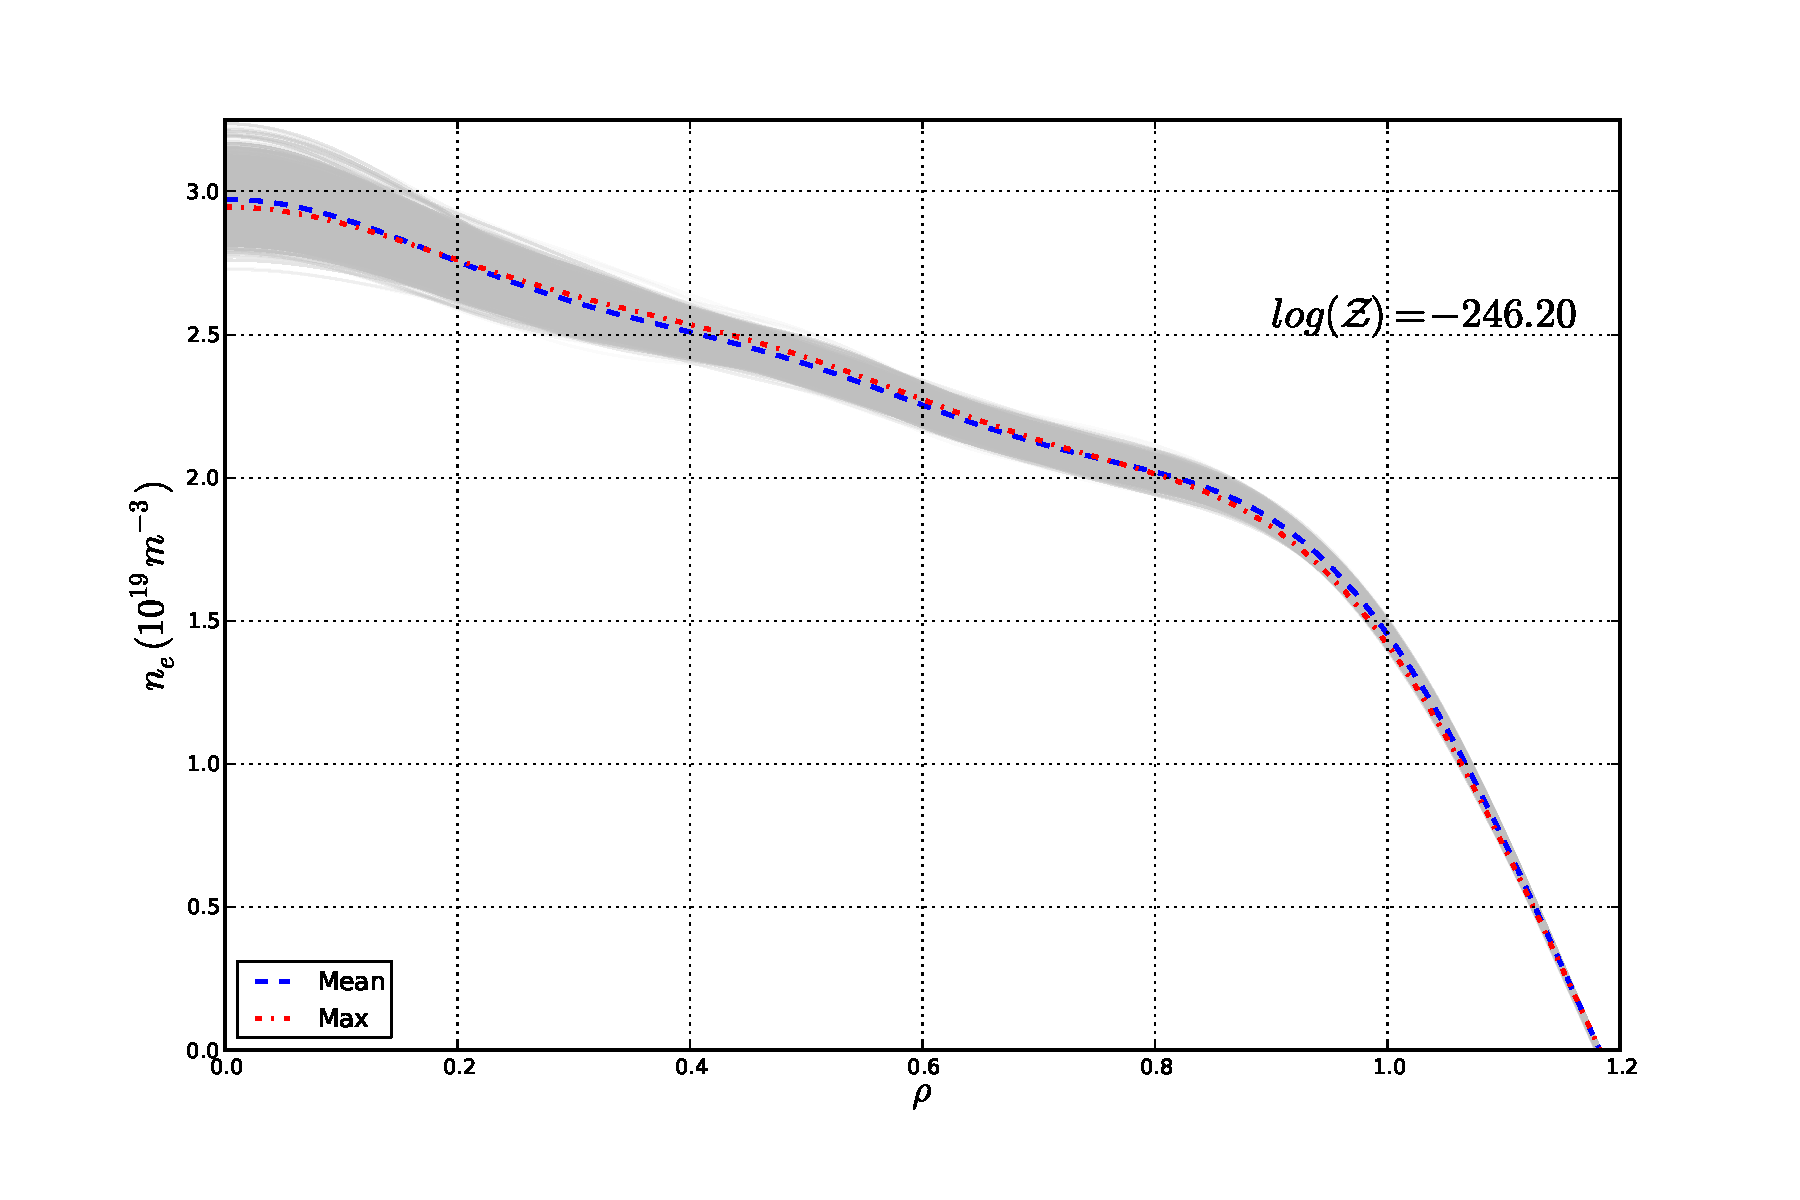
\includegraphics[width=12cm,keepaspectratio=true]{figures/bfit146102_00505_all5}
	\vspace{-30pt}
	\caption{Reconstruction}
\end{figure}
otherstuff
\subsection{L-mode reconstruction}
stuff
\section{Representation of Error}
stuff
\section{Determining discrepant diagnostics}
\begin{figure}[h]
	\centering
	\begin{subfigure}[b]{0.5\textwidth}
		\centering
		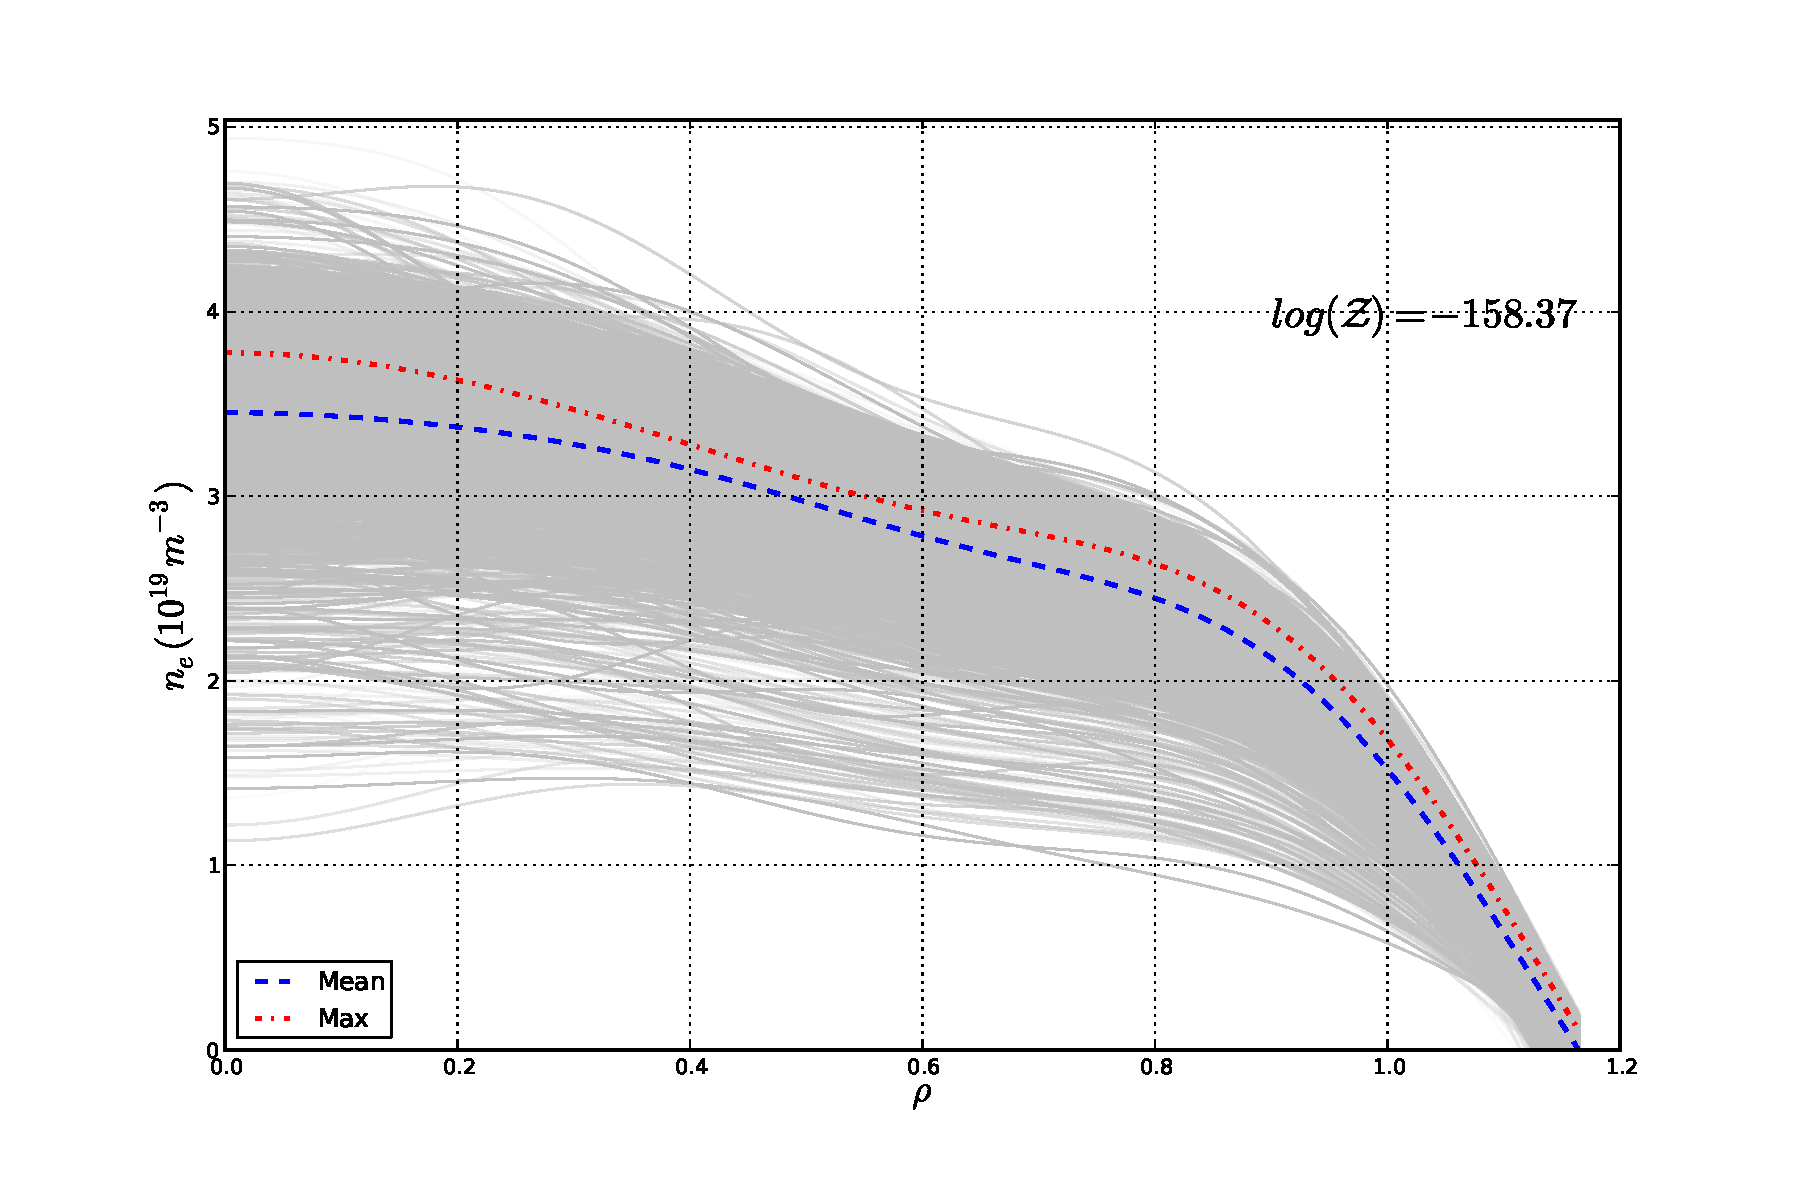
\includegraphics[width=\textwidth,keepaspectratio=true]{figures/bfit146102_00505_thom5}
		\vspace{-30pt}
		\caption{Thomson scattering}
		\label{fig:ts505}
	\end{subfigure}
	\hspace{-20pt}
	\begin{subfigure}[b]{0.5\textwidth}
		\centering
		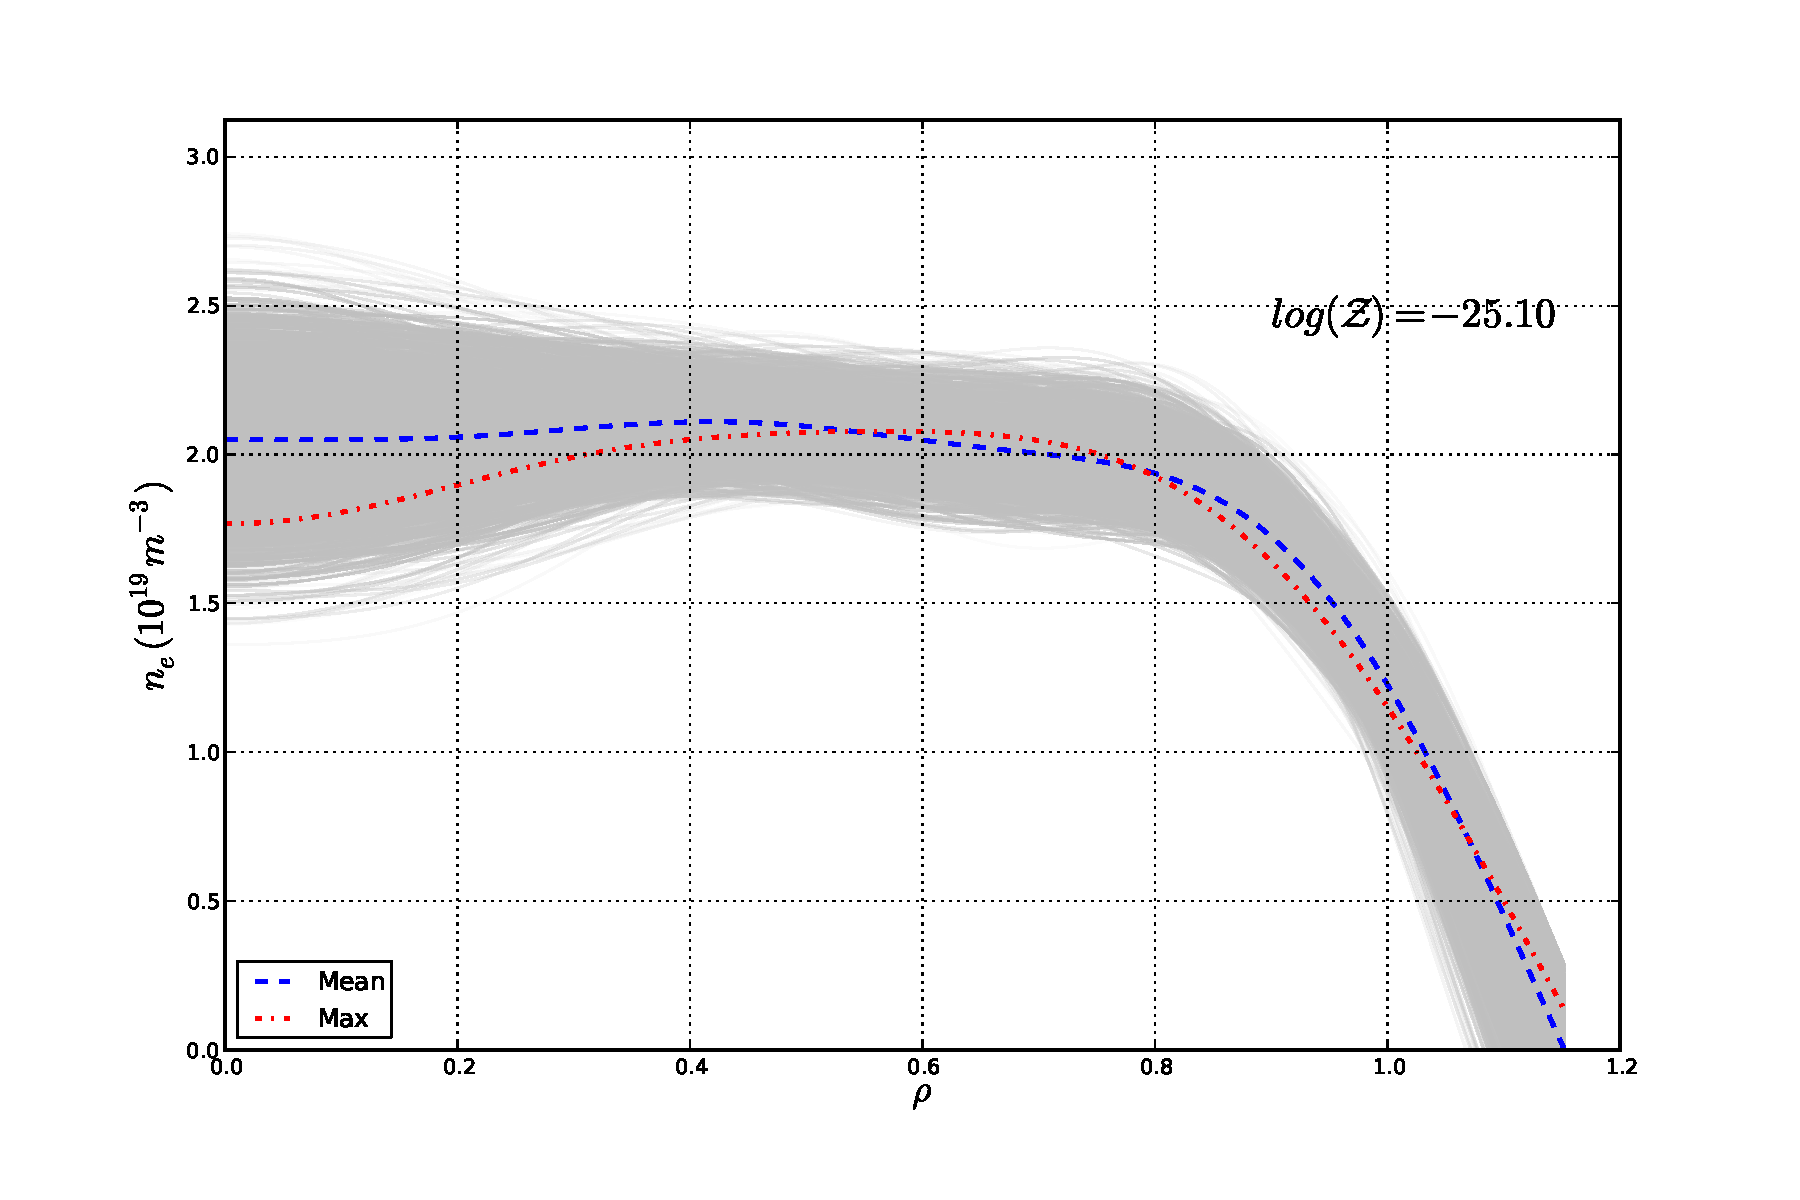
\includegraphics[width=\textwidth,keepaspectratio=true]{figures/bfit146102_00505_inter5}
		\vspace{-30pt}
		\caption{Interferometer}
		\label{fig:inter505}
	\end{subfigure} \\%  ------- End of the first row ----------------------%
	\begin{subfigure}[b]{0.5\textwidth}
		\centering
		\includegraphics[width=\textwidth,keepaspectratio=true]{figures/bfit146102_00505_refl5}
		\vspace{-30pt}
		\caption{Reflectometry}
		\label{fig:refl505}
	\end{subfigure}
	\hspace{-20pt}
	\begin{subfigure}[b]{0.5\textwidth}
		\centering
		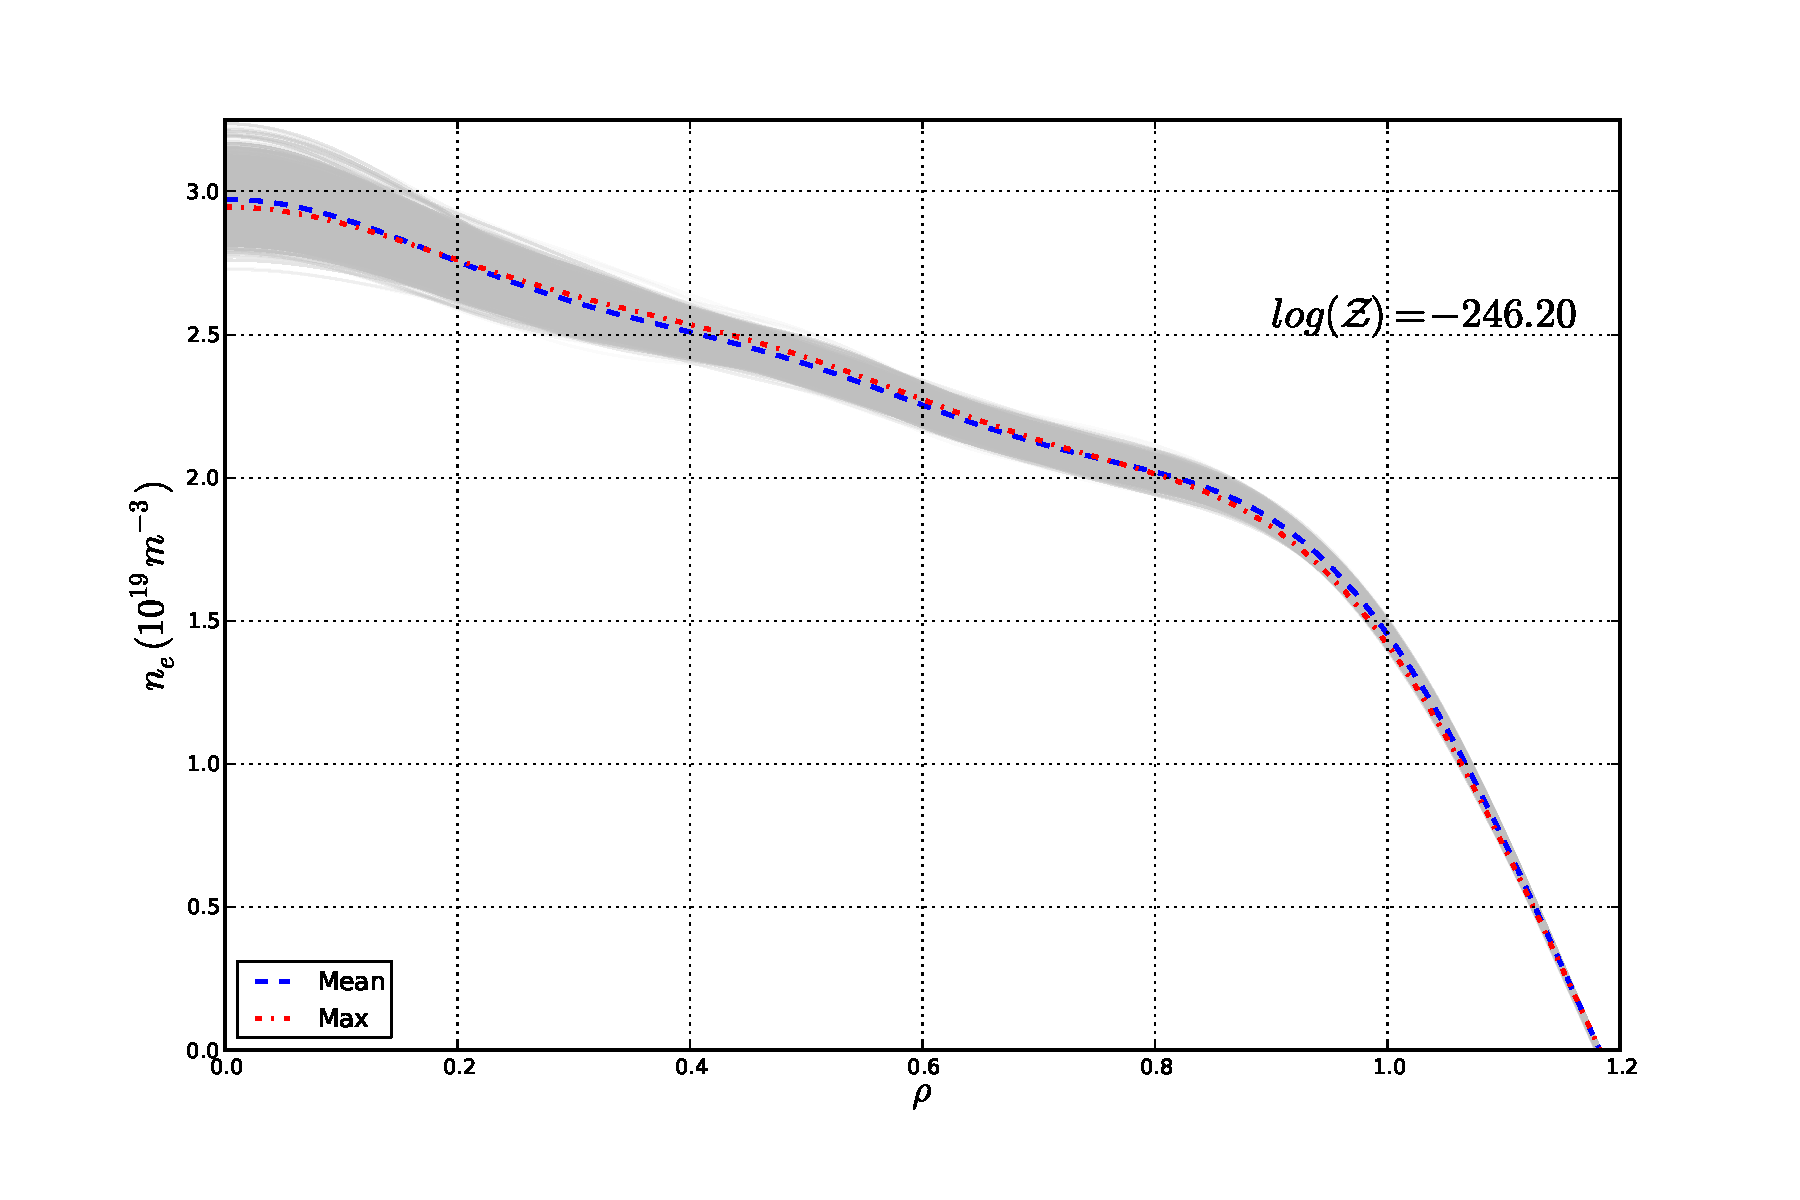
\includegraphics[width=\textwidth,keepaspectratio=true]{figures/bfit146102_00505_all5}
		\vspace{-30pt}
		\caption{Combined}
		\label{fig:all505}
	\end{subfigure}
	\caption{The l-o-n-g caption for all the subfigures (FirstFigure through FourthFigure) goes here.}
	\label{fig:dne505}
\end{figure}
stuff
\section{Conclusions and future work}
stuff
\newpage
\bibliographystyle{unsrt}
\bibliography{bayes,algorithms,diag}
\end{document}
